\chapter{Research And Approach}\label{ch:approach}
In this chapter we will cover the process of building the desired syntax of our language, and research into the domain.

The end goal of this chapter is to have ``working'' scripts for selected use cases.
The following chapter will then cover implementing the compilation of these scripts.


\section{Example Use Cases}\label{sec:example-use-cases}
To have a better understanding of the desired functionality of our language, we define several use cases that our
solution may be applied to.

Throughout this section we will be defining specific functions that we envision being used, and what must be exposed to
comfortably support them.
It should be noted that for many use cases, we will be drawing from real world algorithms, as for most of these
algorithms there already exist solutions - our goal will not be to implement them ourselves, but to provide a platform
where they can be executed.
For example, in~\ref{subsec:naive-pathfinding} we cover our need for a pathfinding algorithm, here we are referring to
being able to build a domain where the information can exist, in reality if we implement an algorithm such as djikstra
search, we will simply be passing the values we have procured into an imported library.

\subsection{Minimum Viable Product}\label{subsec:minimum-viable-product}
For the language to be usable it must implement basic types and operations, as the focus of the language, graphs must
exist as a data type that can be created and modified.
Ideally our MVP would include a turing complete~\cite{TuringCompleteness} suite of operations, allowing users to take
advantage of supported functionalities, while still having the ability to build ad-hoc unsupported features.

\begin{figure}[H]
    \centering
    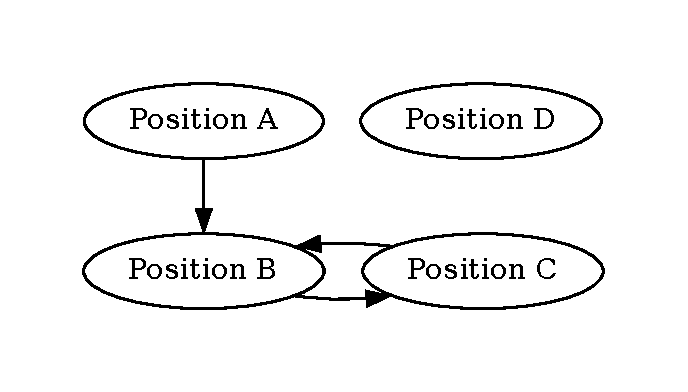
\includegraphics[width=12cm]{figures/example_graphs/basics.gv}
    \caption{An example of a graph displaying each of the most basic features that we expect to implement}
    \label{fig:example_basic_graph}
\end{figure}

Figure~\ref{fig:example_basic_graph} covers the three types of relationships we are expecting to come across.
Our first graph based feature would naturally be to find some way to visualize the graph that we have built, similar to
the generated figure.

TODO: WHAT ARE BASIC LANGUAGE FUNCTIONALITIES TO PUT HERE

\subsection{Naive Pathfinding}\label{subsec:naive-pathfinding}
One of the more fundamental sets algorithms in computing, we expect a finished product to support some level of node
navigation and optimisation.

\begin{figure}[H]
    \centering
    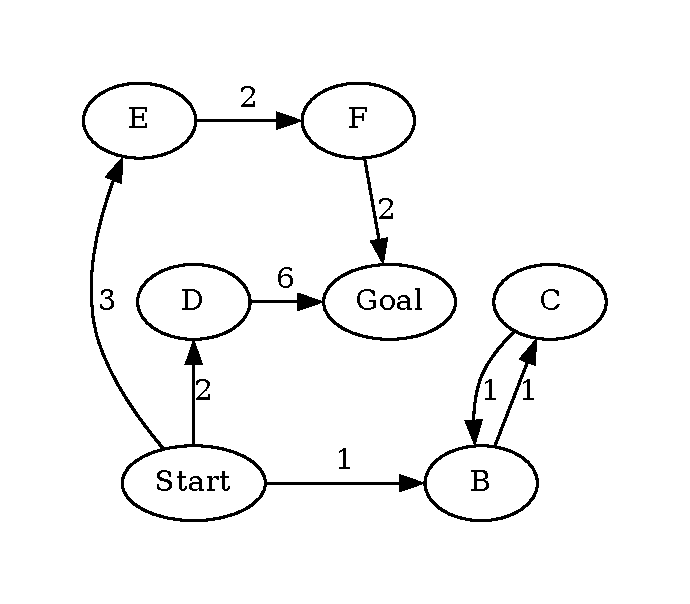
\includegraphics[width=12cm]{figures/example_graphs/pathfinding.gv}
    \caption{An example of a graph that needs to be navigated through}
    \label{fig:example_pathfinding_graph}
\end{figure}

Figure~\ref{fig:example_pathfinding_graph} defines a graph that has a starting node and a goal node, with edges
simulating the cost of traversing between nodes.
Our intent when implementing pathfinding support is to provide a framework where a user can build such a graph, and
given an arbitrary start node, goal node, and algorithm, will be able to retrieve the cost and path that is outputted by
the algorithm.
One important note when implementing such a functionality is that pathfinding algorithms assume a cost of node
traversal, if we build a generalised solution we will have to ask ourselves how this cost should be implemented, as we
have multiple options:

\textbf{All edges have costs, defaulting to 0}~-~this approach allows us to run pathfinding algorithms on any graph, and
requires very little work from a programmer to ensure the graph remains compliant.
However, there are arguments to be made for wasted allocated memory on larger graphs that have no need for such a value.

\textbf{Different subclasses of graphs}~-~this approach would allow us to define a type of graph that MUST have a cost,
while it prevents useless memory allocation, it also requires more work on the side of the developer, who must both
learn and remember the arbitrary definition we have created.

\textbf{Algorithms that treat undefined costs as 0}~-~while this approach may seem more elegant, as it avoids both
previously listed issues, it also introduces implicit functionality, which may produce confusing results if developers
expect a different behaviour when attempting to use pathfinding on non-compliant graphs.

\subsection{Constraint Satisfaction}\label{subsec:constraint-satisfaction}
Constraint satisfaction allows developers to create nodes as a set of domains that can then be reduced.
Creating a graph that needs to be constrained requires us to define two features - a node must be comprised of a domain
of possible values (that will then be constrained); and the constraint itself must exist as part of the relationship.
Unary constraints must also be taken into consideration, as they do not require a relationship to exist.

\begin{figure}[H]
    \centering
    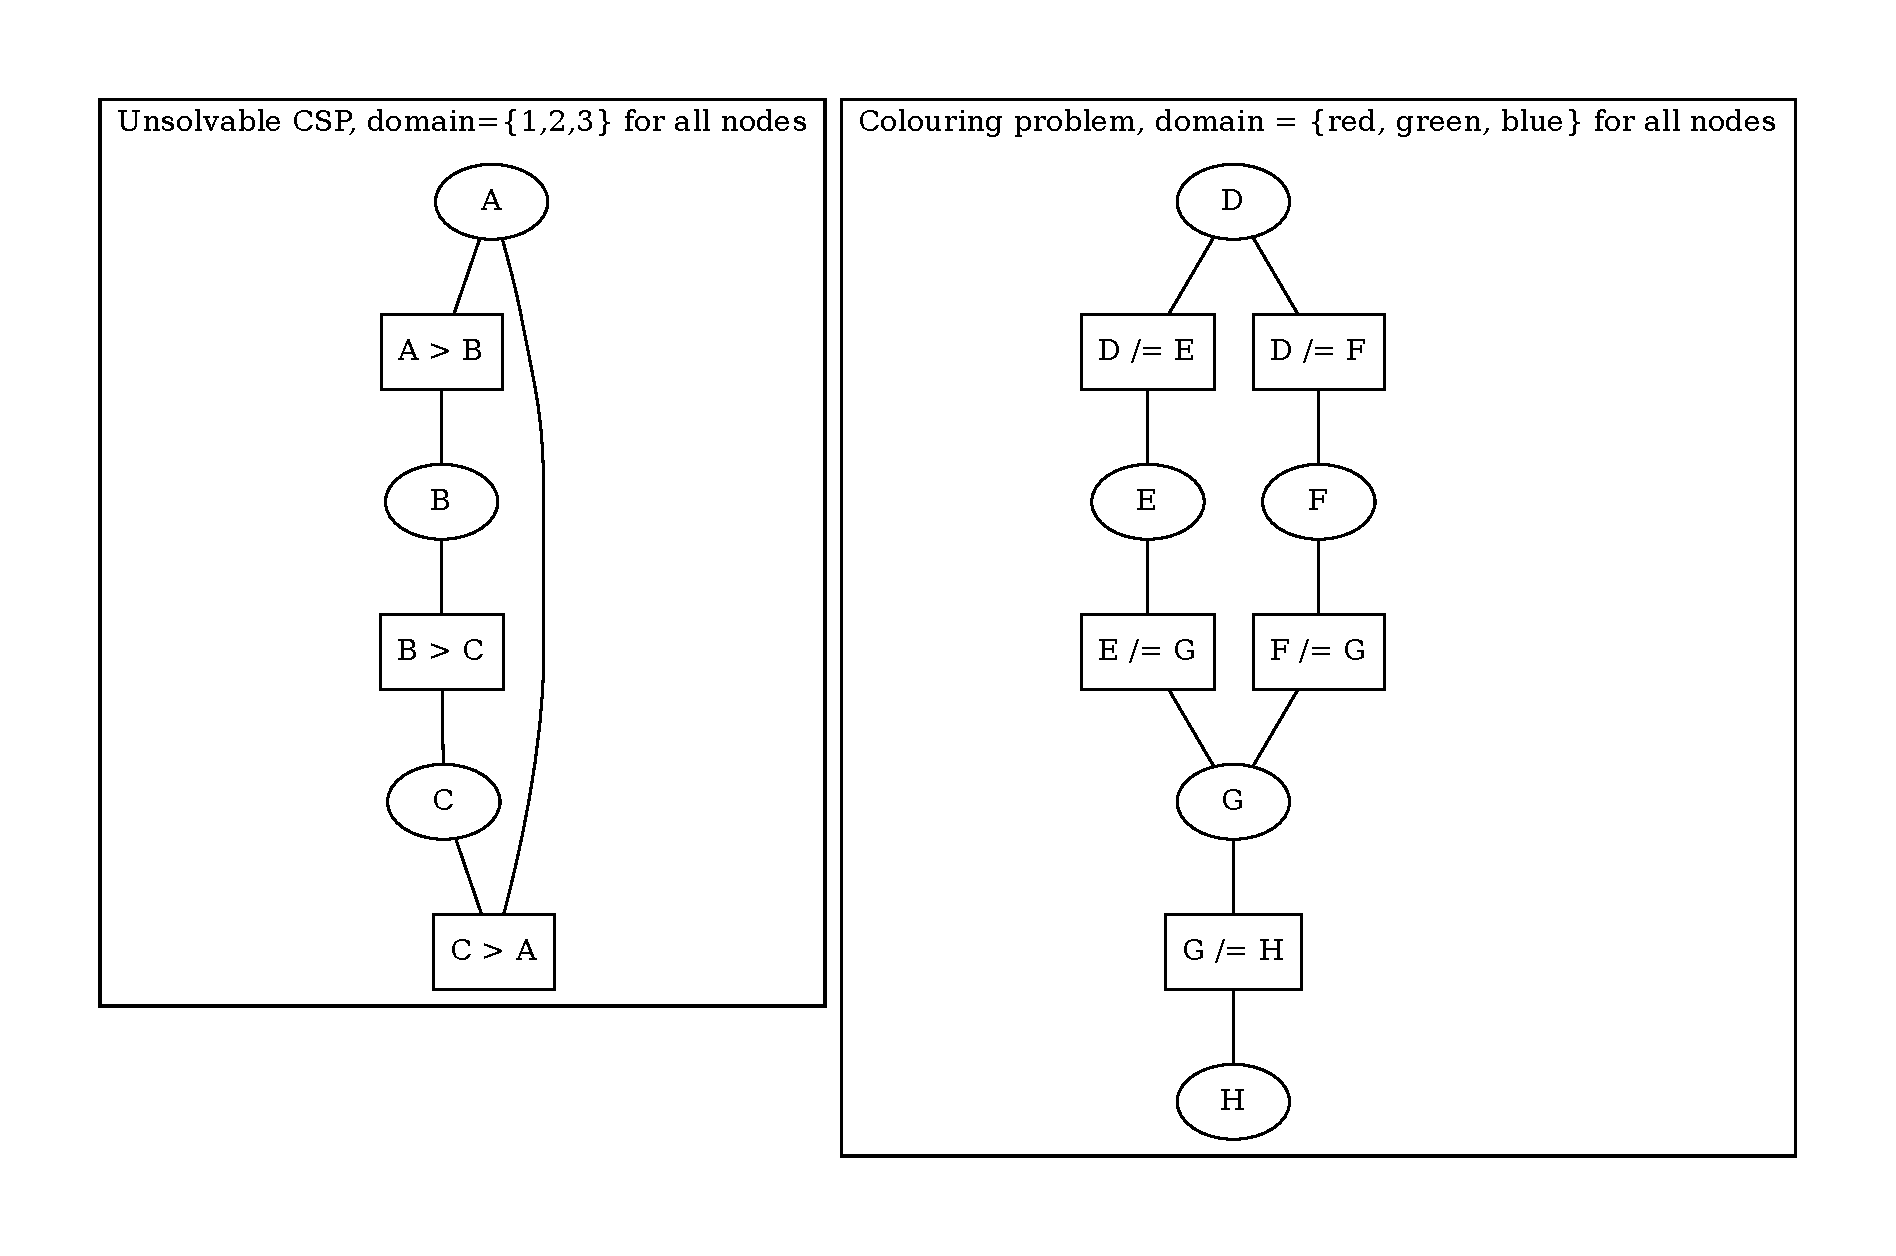
\includegraphics[width=12cm]{figures/example_graphs/constraint_satisfaction.gv}
    \caption{An example of a graph has constraints that need to be acted upon}
    \label{fig:example_constraint_graph}
\end{figure}

In Figure~\ref{fig:example_constraint_graph} we define two separate graphs that can be constrained.
Our first consideration for the first graph is how our language should respond to situations where constraints can not
be met, we will discuss this in further detail during the implementation section.
Next, we approach a more realistic constraint problem with applicable algorithms to find a list of ``correct'' answers.
Here we run into similar questions as were raised in pathfinding, how do we handle knowing whether a graph is compliant
with required format for CSP algorithms?

Lastly we introduce the possibility of interoperability between constraint satisfaction and other language features.
As constraints remove items from a domain, we can introduce the concept of changing or adding constraints as a form
of modifying existing data.
A common use case may be that to remove a node, it would simply have a unary constraint applied to it which is always
False - alternatively it may make more sense to introduce variable elimination functionality to ensure that changes
remain predictable.

\subsection{Trees}\label{subsec:trees}
Trees can be considered a subset of graphs, in that they limit the way relationships can be formed.
Earlier we mentioned the possibility of inherited types that can be used to ensure specific structures - for trees we
believe that this distinction is necessary, as it is a significant departure from what a graph can represent.

\begin{figure}[H]
    \centering
    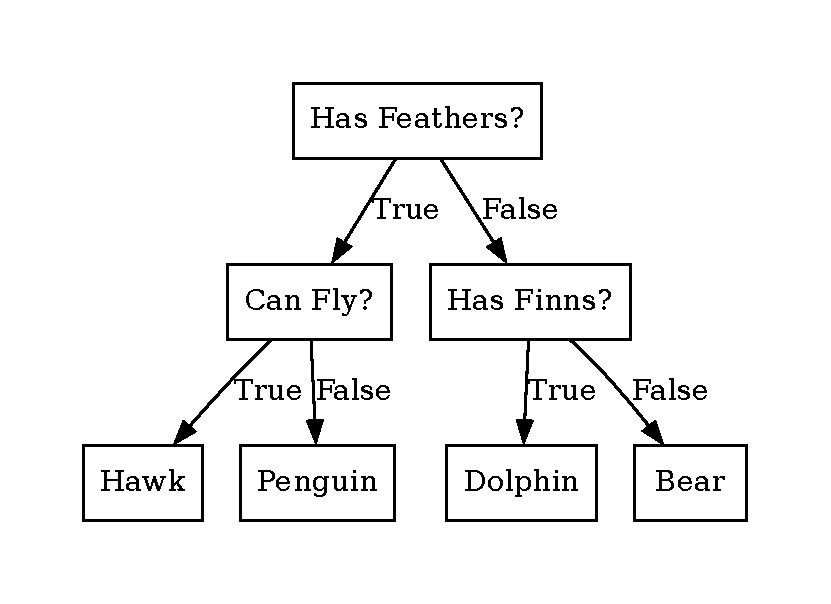
\includegraphics[width=12cm]{figures/example_graphs/decision_tree.gv}
    \caption{An example of a decision tree that could be represented in our language}
    \label{fig:example_decision_tree}
\end{figure}

In figure~\ref{fig:example_decision_tree} we define a basic tree structure, logically, it appears that the only
consideration we will have when building this structure is to ensure that nodes may only be added or removed in a
certain way.
Unlike previous sections we do not run into ill-formed algorithms here, any solution that applies to the previous
sections will be inherited into this section.

\subsection{Complex Use Cases}\label{subsec:complex-use-cases}
p2p net topology
neural nets
graph database

\subsection{Feature Wishlist}\label{subsec:feature-wishlist}
In conclusion to covering use cases we can draw a prioritised list of features that we would want to include in our
language, this will help us with our preliminary research into the tools and approaches we will need to implement.

The features as a rough overview are as follows:
\begin{itemize}
    \item Basic language functionalities
    \item The ability to build a graph data type with Nodes connected by Edges
    \item Functionality to apply basic CRUD operations on nodes and edges
    \item Functionality to find optimal paths between nodes
    \item Functionality to constrain nodes by building constraints along edges (or on nodes for unary constraints)
\end{itemize}


\section{Technologies}
In this section we will cover the technologies that will be involved in the final product.

\subsubsection{Language Considerations}
Before creating any code we have two language considerations to make.

The first consideration is the language to use for the compiler;
A good compiler tool is sufficiently portable that it is not difficult to use on any type of machine, historically this
has always been an issue, as Operating Systems and computer architecture have a wide variety - therefore the language
we use must be capable of creating executables for such a wide variety of systems.
In addition, as development time is significant, we should choose a language that provides sufficient tooling to
minimise unnecessary development time.

Our choice of compiler language is C#, due to its wide system compatibility and support of the~\cite{ANTLR} which we
will explore later.

Next we have to decide what language to compile to, which entails similar considerations as the user will want an
executable that requires minimal to no tweaking.
For this decision we have taken a slightly different approach - in order to fully leverage the language that we compile
to, we plan to support code injection - for this to remain convenient it's better to choose a language that more closely
resembles the one we're translating from.

In this train of thought, we have decided to compile to python, as it is a similarly high level language to the one
we are designing.

\subsubsection{Compiler Tools}\label{subsubsec:compilertools}
Our choice for compiler tooling follows a similar logic to most development tools, we would like ease of use, while
maintaining support for more complex functionality.

The main decision that had to be made was between ANTLR and leveraging the toolkit that intellij
provides~\cite{IntellijLanguage}.
After choosing ANTLR, we reasoned that we could take advantage of the parse tree that ANTLR creates for both debugging
and traversal properties - as ANTLR creates an easily readable image displaying how the grammar operates.
Furthermore, ANTLR introduces with it the listener pattern~\cite[p18]{ANTLRReference}

The document describing the syntax and semantics of a language is referred to as a ``grammar''\cite{Grammars}, both
ANTLR and the intellij plugin are based on Extended Backus-Naur Form (EBNF), they also both include a feature for
regex injection - allowing more well-formed rules to be written using fewer lines of code.

\subsubsection{Language Tools}
For the purpose of having usable output, we have decided to visualise the graphs we build.
The tool we'll be using for this purpose is GraphViz\cite{GraphViz} - which takes advantage of standardised grammar
called the DOT language, that can be used to consistently generate the same image.
Graphviz has a python library, so we can easily incorporate it into the print statements we define.
%
%
%\section{Syntax}\label{sec:syntax}
%The most visible part of any language is its syntax.

In this section we will try to reach a conclusion for what operations we would like to implement and the syntax
that we believe they should be represented by.

Our end goal will be to have a guideline for what operations are represented as, though they may have to be tweaked
during implementation if we find issues.

\bigskip

\noindent
When defining syntax we try to keep the following in mind:

\noindent
\textbf{Popularity} \- \textit{do other languages use this notation?}

If the notation is already popular then it will be less confusing for experienced programmers to learn

\noindent
\textbf{Verbosity} \- \textit{how obvious is the operator?}

If we create notation that doesn't feel natural, it might lead to a lot of unnecessary documentation reading

\noindent
\textbf{Obscurity} \- \textit{is the operator too similar to existing operators?}

If so, programmers may be confused what is occurring in existing code, causing it to take longer to debug

\subsection{Ambigouty in Ownership and Operation}
context vs explicit operations.

\subsection{Assignment and Types}
The most simple operation we can perform is assignment, as we have chosen to build a strongly typed language, we will
specify explicit definitions using the popular {type} {var_name} = {value}

\subsection{Branching}
if else

\subsection{Graphs}
include inheritance option.

\subsection{Nodes}
ref and clone and immutability.


\subsection{Unique Operators}
why we agree these obscure operators are fair tradeof

\subsection{Edges}
operators on edges.
rel keyword.
terms
TODO: decide if you're happy with this order


\subsection{Iteration}
while + fmap

\subsection{Polymorphic Implications}
runtime checks, var and node operations.

\subsection{Semantic Ambigouities Arising From the Syntax}
Insert some examples here from the discussion.
%
%\section{Context-Free Grammar}\label{sec:grammar}
%To specify some rules about how a program in Lattice should be composed, we have written the following context-free grammar, using Extended Backus-Naur form.
This grammar can then be used to build a parser and recognize valid Lattice programs and their structure.

\subsubsection*{Global composition of a program}

A program in Lattice would be a sequence of statements and function definitions.

\begin{align*}
    \mathit{Start} \rightarrow \{ \mathit{FunctionDef} \mid \mathit{Statement} \}
\end{align*}
\captionedgrammar{Description of the global structure of a program}

Statements can be variable declarations, variable assignments, graph manipulation (i.e.\ opening a graph context to do operations), print statements, blocks of code in an if-else control structure or a while loop, or a return statement.

\begin{align*}
    \omit $\mathit{Statement}$ \hfil& \rightarrow \mathit{VarDecl} \\
    & \mid \mathit{VarAssignOrGraphManip} \\
    & \mid \mathit{PrintStatement} \\
    & \mid \mathit{IfBlock} \\
    & \mid \mathit{WhileBlock} \\
    & \mid \mathit{ReturnStatement}
\end{align*}
\captionedgrammar{Description of the different kind of statements}

\subsubsection*{Variable declaration}

A variable is declared by writing its type followed by its name.
After the variable declarations the statement can end with a semicolon or there can be a value assigned to the variable or a graph context can be opened.

There need to be a global production rule for variable assignment and graph manipulation because both statements start with a variable identifier so having the rules be fully separated would mean that the grammar isn't LL(1).
Once the variable for which we are writing the statement is specified, the rest of the statement can either correspond to an assignment or to a block of code in a graph context.

\begin{align*}
    \omit $\mathit{VarDecl}$ \hfil& \rightarrow \mathit{Type} \: \text{varId} \: \mathit{VarDeclTail} \\
    \omit $\mathit{VarDeclTail}$ \hfil & \rightarrow \mathit{TailVarAssignOrGraphManip} \\
    & \mid \text{semicolon} \\
    \omit $\mathit{VarAssignOrGraphManip}$\hfil & \rightarrow \text{varId} \: \mathit{TailVarAssignOrGraphManip} \\
    \omit $\mathit{TailVarAssignOrGraphManip}$ & \rightarrow \mathit{TailVarAssign} \\
    & \mid  \mathit{TailGraphManip}\ \\
    \omit $\mathit{Type}$ \hfil & \rightarrow \text{typeString} \\
    & \mid \text{typeFloat} \\
    & \mid \text{typeBool} \\
    & \mid \text{typeInt}\\
    & \mid \text{typeGraph}
\end{align*}
\captionedgrammar{Rules for variable declaration}

\subsubsection*{Variable assignment and arithmetic expressions}
To assign a value to a variable, the variable name needs to be followed by the assignment operator and then the assigned value, which can be a string, a boolean value, an arithmetic expression with variables, numbers and function calls or simply a function call, a number or another variable.

\begin{align*}
    \omit $\mathit{TailVarAssign}$ \hfil & \rightarrow \text{opAssign} \: \mathit{AssignVal} \: \text{semicolon} \\
    \omit $\mathit{AssignVal}$ \hfil & \rightarrow \text{string} \\
    & \mid \mathit{Expr} \\
    & \mid \mathit{BoolVal}\\
    \omit $\mathit{Expr}$ \hfil & \rightarrow \text{opSub} \: \mathit{Expr} \\
    & \mid \mathit{Expr} \: \mathit{MulOp} \: \mathit{Expr} \\
    & \mid \mathit{Expr} \: \mathit{AddOp} \: \mathit{Expr} \\
    & \mid \text{leftParen}\: \mathit{Expr} \: \text{rightParen} \\
    & \mid \mathit{Number} \\
    & \mid \text{varId} \\
    & \mid \mathit{FuncCall} \\
    & \mid \text{KeywordFmap} \: \text{varId} \: \text{varId} \\
    \omit $\mathit{BoolVal}$ \hfil & \rightarrow \text{keywordTrue} \\
    & \mid \text{keywordFalse} \\
    \omit $\mathit{Number}$ \hfil & \rightarrow \text{integer} \\
    & \mid \text{floatLit} \\
    \omit $\mathit{AddOp}$ \hfil & \rightarrow \text{opAdd} \\
    & \mid \text{opSub} \\
    \omit $\mathit{MulOp}$ \hfil & \rightarrow \text{opMult} \\
    & \mid \text{opDiv} \\
    & \mid \text{opRem}
\end{align*}
\captionedgrammar{Rules for variable assignment and arithmetic expressions}

This definition of the grammar has a lot of rules but doesn't allow the precedence of arithmetic operations to be handled during the building of the parse tree and makes the grammar ambiguous.
However, those rules allow us to have the desired behavior when we use the tool we have chosen for the implementation (\ref{TODO}).

\subsubsection*{Graph Manipulation}

After having specified the graph context in which we want to work, we can do graph-specific operations as well as the other ones.

\begin{align*}
    \omit $\mathit{TailGraphManip}$ \hfil &\rightarrow \text{leftBrace} \: [\mathit{ListGraphOp}]  \: \text{rightBrace} \\
    \omit $\mathit{ListGraphOp}$ \hfil &\rightarrow \mathit{graphOp} \: \mathit{ListGraphOp} \\
    \omit $\mathit{GraphOp}$ \hfil &\rightarrow \mathit{AddRel}  \\
    & \mid \mathit{AddClone} \\
    & \mid \mathit{AddRef} \\
    & \mid \mathit{Statement} \\
    \omit $\mathit{AddRel}$ \hfil & \rightarrow \text{varId opRelLeft} \: \mathit{Number} \: \text{comma string opRelRight varId} \\
    \omit $\mathit{AddClone}$ \hfil & \rightarrow \text{keywordClone varId semicolon} \\
    \omit $\mathit{AddRef}$ \hfil & \rightarrow \text{keywordRef varId semicolon}
\end{align*}
\captionedgrammar{Rules regarding graph contexts}

\subsubsection*{Print statement}

The print function is quite minimalist and can only be used for strings and variables, using the keyword $\texttt{print}$.

\begin{align*}
    \mathit{PrintStatement} \rightarrow \text{keywordPrint} \: (\text{varID} \mid \text{string}) \: \text{semicolon}
\end{align*}
\captionedgrammar{Structure of a print statement}

\subsubsection*{If-else statement}

The if-else statement structure is quite classic.
After the \texttt{if} keyword, a boolean expression is specified between parenthesis and then the block of code to execute is written between curly brackets.
The following else clause is optional.

\begin{align*}
    \omit $\mathit{IfBlock}$ \hfil &\rightarrow \mathit{IfClause} \: [\mathit{ElseClause}] \\
    \omit $\mathit{IfClause}$ \hfil &\rightarrow \text{keywordIf} \: \text{leftParen} \: \mathit{BoolExpr} \: \text{rightParen} \: \text{leftBrace} \: \{ \mathit{statement}\} \: \text{rightBrace} \\
    \omit $\mathit{ElseClause}$ \hfil &\rightarrow \text{keywordElse} \: \text{leftBrace} \: \{ \mathit{statement} \} \: \text{rightBrace} \\
    \omit $\mathit{BoolExpr}$ \hfil &\rightarrow \text{opBNot} \: \mathit{BoolExpr} \\
    & \mid \mathit{BoolExpr} \: \mathit{BoolOp} \: \mathit{BoolExpr} \\
    & \mid \mathit{AssignVal} \: \mathit{CompOp} \: \mathit{AssignVal} \\
    & \mid \text{leftParen} \: \mathit{BoolExpr} \: \text{RightParen} \\
    & \mid \text{varID} \\
    & \mid \mathit{FuncCall} \\
    & \mid \mathit{BoolVal} \\
    \omit $\mathit{BoolOp}$ \hfil &\rightarrow \text{opBAnd} \\
    & \mid \text{opBOr} \\
    \omit $\mathit{CompOp}$ \hfil & \rightarrow \text{opBEq} \\
    & \mid \text{opBNeq} \\
    & \mid \text{opBGrt}
\end{align*}
\captionedgrammar{Rules for if-else statements and boolean expressions}

Since the boolean expression and the arithmetic expression are different, writing an arithmetic expression as the condition of an $\texttt{if}$ statement is a syntax error, not a type error that would be found by the type checker or a semantic error despite what some people might expect.
This distinction also causes our grammar to be bigger complicating the implementation part.
We still made the choice to write our grammar that way because the tool we use gives this grammar some redeeming qualities (\ref{TODO})

\subsubsection*{While loop}

The while loop isn't original either.
The statement starts with the keyword \texttt{while} followed by the condition for the loop and then the block of code to repeat.

\begin{align*}
\mathit{WhileBlock} &\rightarrow \text{keywordWhile} \: \text{leftParen} \: \mathit{BoolExpr} \: \text{rightParen} \: \text{leftBrace} \: \{ \mathit{statement}\} \: \text{rightBrace}
\end{align*}
\captionedgrammar{Description of a while loop}

\subsubsection*{Function definition and function call}

Function definitions are introduced with the keyword $\texttt{def}$, followed by the name of the function, the types and names of the arguments and then the block of code executed by the function.
The keyword $\texttt{def}$ allows to distinguish the function declaration from a variable declaration because otherwise both statements would start with a type token.
It is possible to have a rule for both statements, as with the $\mathit{VarAssignOrGraphManip}$ rule, but that would mean that function declaration has the same rules as any statement and we couldn't use the grammar to enforce that function declaration can't be done in a $\texttt{while}$ or $\texttt{if-else}$ block of code.\\

A return statement is necessary to write a function so there is a rule describing it.
However, the parser can't enforce that necessity to have a return statement in a function, because it could be written in an $\texttt{if-else}$ block of code which makes it indistinguishable from standard statement.

Once defined, the function can then be called in the contexts mentioned above, by writing the function name and the parameters.

\begin{align*}
    \omit $\mathit{FuncDef}$ \hfil &\rightarrow \text{keywordDef} \: \mathit{Type} \: \text{varID leftParen} [\mathit{ListArgs}] \text{rightParen} \\
    & \text{leftBrace} \: \{ \mathit{statement} \} \: \text{rightBrace} \\
    \omit $\mathit{ListArgs}$ \hfil &\rightarrow \mathit{Arg} \:  \mathit{TailListArgs} \\
    \omit $\mathit{Arg}$ \hfil &\rightarrow \mathit{Type} \: \text{varId} \\
    \omit $\mathit{TailListArgs}$ \hfil & \rightarrow \{ \text{comma} \: \mathit{Arg} \} \\
    \omit $\mathit{ReturnStatement}$ \hfil &\rightarrow \text{keywordReturn} \: \mathit{AssignVal} \: \text{semicolon} \\
    \omit $\mathit{FuncCall}$ \hfil &\rightarrow \: \text{varID leftParen} [\mathit{ListParam}] \: \text{rightParen} \\
    \omit $\mathit{ListParam}$ \hfil &\rightarrow \mathit{varID} \:  \{ \text{comma} \: \mathit{varID} \}
\end{align*}
\captionedgrammar{Rules for function definitions and function calls}


%
%\section{Semantics}\label{sec:semantics}
%This section will be used to comprise the sets of semantic rules we intend to follow throughout the project.
It should be noted as we have no formal semantic definition, we must test and ensure these rules throughout the
compiler.

\subsubsection{Variable declaration, assignment, and access}

\begin{itemize}
    \item Each variable must be declared before being assigned a value.
    \item Each variable must have a unique name throughout the program, regardless of the scope.
    \item Variables must be initialized with a value before they are accessed (for example in an expression or function call).
    \item The value assigned to a variable must be compatible with its declared type.
\end{itemize}

\subsubsection{Type rules}

\begin{itemize}
    \item Assignment from float to integer is not allowed, but assignment from integer to float is allowed.
    \item Arithmetic expressions involving integers and floats will result in a float value.
    \item Arithmetic expressions with strings are not allowed.
    \item Boolean expressions can compare floats and integers and the result of \texttt{2.0 == 2} is true.
    \item Comparisons must be made between compatible types.
    \item String comparisons are limited to equality checks; the greater than operator is not applicable.
    \end{itemize}

\subsubsection{Functions}

\begin{itemize}
    \item A function needs to be defined before being called.
    \item The type and number of arguments in a function call must match the declared function signature.
    \item The return statement is only allowed within the scope of a function.
    \item All functions must have unique names.
    \item The value returned by a function must match its declared return type.
    \end{itemize}

\subsubsection{Graph contexts}

\begin{itemize}
    \item A variable needs to be referenced in a context before it can be used in relations or other statements in this context, even if it was first declared in this context.
\item A variable can only be referenced or cloned in a context if it is present (declared or referenced) in the parent context.
    \item Printing a graph will display its nodes and relations as well as the ones in the child graph contexts if there are any.
    \item There can be any number of relation between two nodes, the weight,label and direction of the edge don't have to be unique.
    \item The variable on which the \texttt{fmap} statement is applied must be a graph
    \item The type of all the nodes in a graph must match the one of the parameters of the function called with the \texttt{fmap} keyword.
    \item The function called with the \texttt{fmap} keyword must have only one parameter.
    \end{itemize}


